\documentclass{sysuthesis}
\usepackage{verbatim}
%%
% 论文相关信息
% 本文档中前缀"c-"代表中文版字段, 前缀"e-"代表英文版字段
% modifyer: 黄俊杰(huangjj27, 349373001dc@gmail.com)
% update date: 2017-04-13
%%

% 标题
% 论文题目应以简短、明确的词语恰当概括整个论文的核心内容,避免使用不常见的缩略词、缩写字。读者通过标题可大致了解毕业设计(论文)的内容、专业的特点和科学的范畴。中文题目一般不宜超过 24 个字,必要时可增加副标题。外文题目一般不宜超过 12 个实词

% 封面标题。由于技术所限,封面题目过长的划分交由用户您进行定夺
% 这也能让您的论文封面看起来更有美感
\covertitlefirst{“鲜天下”平台}
\covertitlesecond{系统分析与设计方案}

% Author:   Souler Ou
% 修改者:    欧一锋
% Date:     3/30/2018
% Mail:     ou@souler.cc
%如果英文标题过长可以使用此两项作为表三(答辩记录表)的标题。
\etitlefirst{Unofficial \Latex\ Template}
\etitlesecond{for SYSU Graduation Thesis}

% 另外一种封面的论文题目. 换行使用换行符("\\")
%\title{
%    中山大学 \\
%    本科毕业论文非正式模版
%}

% 中文标题
\ctitle{“鲜天下”平台-系统分析与设计方案}
\etitle{Unofficial \LaTeX\ Template for Undergraduate Thesis of SYSU}

% 解决英文摘要页标题过长问题 (Issue 49&63)
% 当\etitle的长度超过页边距时,请使用下面的命令自行断行
% 此操作只影响英文摘要页的标题,不影响页眉的标题
% 如果不需要断行,将\eabstracttitlesecond{ }留空即可
\eabstracttitlefirst{Unofficial \LaTeX\ Template} 
\eabstracttitlesecond{for SYSU Graduation Thesis}

% 作者详细信息
\author{李沐晗\ 颜彬\ 何冠岚\ 张家豪\ 王永锋}
\cauthor{李沐晗\ 颜彬\ 何冠岚\ 张家豪\ 王永锋}    % 封面作者
\eauthor{Chen Guanying}
\studentid{TODO}
\cschool{数据科学与计算机学院}

\cmajor{计算机科学与技术}
\emajor{Computer Science}

% 指导老师
\cmentor{衣杨\ 副教授}
\ementor{A.P. Yi Yang}

     % 论文相关信息
% %%
% 摘要信息
% 本文档中前缀"c-"代表中文版字段, 前缀"e-"代表英文版字段
% 摘要内容应概括地反映出本论文的主要内容,主要说明本论文的研究目的、内容、方法、成果和结论。要突出本论文的创造性成果或新见解,不要与引言相 混淆。语言力求精练、准确,以 300—500 字为宜。
% 在摘要的下方另起一行,注明本文的关键词(3—5 个)。关键词是供检索用的主题词条,应采用能覆盖论文主要内容的通用技术词条(参照相应的技术术语 标准)。按词条的外延层次排列(外延大的排在前面)。摘要与关键词应在同一页。
% modifier: 黄俊杰(huangjj27, 349373001dc@gmail.com)
% update date: 2017-04-15
%%

\cabstract{
摘要内容应概括地反映出本论文的主要内容,主要说明本论文的研究目的、内容、方法、成果和结论。要突出本论文的创造性成果或新见解,不要与引言相混淆。语言力求精练、准确,以300—500字为宜。在摘要的下方另起一行,注明本文的关键词(3—5个)。关键词是供检索用的主题词条,应采用能覆盖论文主要内容的通用技术词条(参照相应的技术术语标准)。按词条的外延层次排列(外延大的排在前面)。摘要与关键词应在同一页。
}
% 中文关键词(每个关键词之间用“;”分开,最后一个关键词不打标点符号。)
\ckeywords{本科毕业论文;\LaTeX\ 模板;中山大学}

\eabstract{
英文摘要内容与中文摘要相同,以250—400个实词为宜。摘要下方另起一行注明英文关键词(Keywords3—5个)。
}
% 英文文关键词(每个关键词之间用半角加空格分开, 最后一个关键词不打标点符号。)
\ekeywords{undergraduate thesis, \LaTeX\ template, Sun Yat-Sen University}

     % 摘要内容
\begin{document}
    % 论文前置部分
    \frontmatter
        \pagenumbering{Roman}
        \maketitle    % 封面
        % \makeabstract       % 中英文摘要
        \maketableofcontents        % 目录
        \makelistoffiguretable

    % 论文主体部分
    \mainmatter
        % 引言

        
        % 正文
        %%%%%%%%%%%%%%%%%%%%%%% 需求分析 %%%%%%%%%%%%%%%%%%%%%%%%%%%%%%%%%%%%%%%%%%
\chapter{需求分析}
%定义,过去的研究和现在的研究,意义,与图像分割的不同,going deeper
\label{cha:demand_analysis}
\section{问题陈述}

我们将采用C/S架构,建立一个连接微供应商和订购商之间的一个中间平台“鲜天下”。通过该平台,我们得以实现这样的目标:聚合小生厂商的生产力以满足大厂家的订单需求,规模化效应减少运行成本,通过可靠的授信模型为小生厂商提供合适额度的贷款以解决成本问题。

在订购商对虾有较大的需求时,通过“鲜天下”平台,订购商能够在该平台发起订单并支付定金,并实时查看该订单的提交情况与完成情况,如果订单被平台所接受并完成,订购商需要向平台支付剩余款项。

微供应商可以在“鲜天下”平台上注册申请成为认证微供应商,并能够从平台中获得订单。完成订单后,还能够从平台中得到相应款项。同时,根据自己需要,微供应商还可以从“鲜天下”平台申请不超过信用额度的贷款,以此来解决成本问题。

为确保微供应商与订购商之间的协作安全,平台管理人员会对平台所接收到的来自订购商的订单进行审核,并确定是否接受该订单。若接受该订单,平台需要将该订单拆分成多个小订单,并且推送给合适的小生产商在规定时间内完成。同时,平台还需要监控微供应商完成情况,并及时收取货物并完成订购商的订单要求。为了减少微供应商的生产压力,鼓励更多的微供应商参与到该平台中贡献生产力并获得更高的利润,该平台还会记录微供应商相关数据,并根据这些数据,智能地判断每个微供应商可得到的信用额度,以让微供应商获得贷款,减缓它们的资金压力,释放更多的生产力,同时保证平台资金流的安全与稳定。

“鲜天下”平台运行Unix服务器上,能够自动处理用户的请求,并将相关信息存储于数据库中。由于这些信息涉及订单与资金流,该数据库系统必须保证内部数据的一致性,以保证平台的资金流正常运转。


\section{用例析取}

对国内外研究现状和相关领域中已有的研究成果的简要评述;
\section{用例规约}

\section{补充规约}

\section{术语表}



        \newclearpage
        %%%%%%%%%%%%%%%%%%%%%%% 架构设计 %%%%%%%%%%%%%%%%%%%%%%%%%%%%%%%%%%%%%%%%%%%%%
\chapter{架构设计}

\section{架构描述}

\section{架构图}

\section{关键抽象}
        \newclearpage
        %%%%%%%%%%%%%%%%%%%%%%% 用例分析 %%%%%%%%%%%%%%%%%%%%%%%%%%%%%%%%%%%%%%%%%%%%%
\chapter{用例分析}
	
\section{补充用例规约}
	经过讨论,上文中的用例已经足够详细了,此部分不添加用例规约。
\section{用例中类的析取}
    在第一章给出的用例归约的基础上,我们将挑选其中比较常用和重要的用例来分析,并给出用例的流程图。
    
	\subsection{用户注册用例分析} % (fold)
	\label{sub:用户注册用例分析}
	\begin{enumerate}
		\item \textbf{类的析取} \\
		用户注册用例允许微供应商和采购商在注册页面进行注册,其中包括的实体类、控制类和边界类如下图
		\autoref{fig:class_enroll}。
		\begin{figure}[htp]
		    %\begin{adjustwidth}{-1.5cm}{-1cm}
		    \centering
		    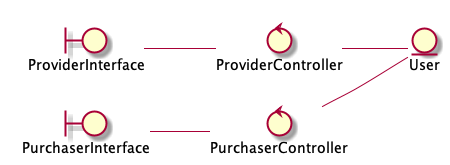
\includegraphics[width=12cm]{report/figure/classAnalyse/enroll.png}
		    \caption{注册用例析取图}
		    \label{fig:class_enroll}
		    %\end{adjustwidth}
		\end{figure}

		\item \textbf{用例工作时序图} \\
		注册用例需要用户在前端打开注册页面,填写信息后通过前端发送给后端,后端进行数据库操作后返回结果,具体流程如下图所示。正确的返回结果应该是待审核或注册失败。义微供应商的注册过程为例,其注册用例实现细节可见\autoref{fig:sd_enroll}。

		\begin{figure}[htp]
		    %\begin{adjustwidth}{-1.5cm}{-1cm}
		    \centering
		    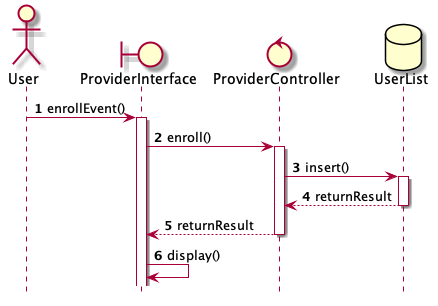
\includegraphics[width=12cm]{report/figure/sequenceDiagram/sd_enroll.png}
		    \caption{用户注册用例工作时序图}
		    \label{fig:sd_enroll}
		    %\end{adjustwidth}
		\end{figure}

	\end{enumerate}
	% subsection 用户注册用例分析 (end)

    \newpage
	\subsection{用户登录用例分析} % (fold)
	\label{sub:用户登录用例分析_name}
	\begin{enumerate}
		\item \textbf{类的析取} \\
		用户登录用例允许管理员、微供应商和采购商这三个类型的用户在登录页面进行登录,其中包括的实体类、控制类和边界类如下图
		\autoref{fig:class_login}.
		\begin{figure}[htp]
		    %\begin{adjustwidth}{-1.5cm}{-1cm}
		    \centering
		    
\includegraphics[width=12cm]{report/figure/classAnalyse/login.png}
		    \caption{用户登录用例析取图}
		    \label{fig:class_login}
		    %\end{adjustwidth}
		\end{figure}
		\item \textbf{登录用例时序图} \\
		登录用例需要用户在前端打开注册页面,填写信息后通过前端发送给后端,后端进行数据库操作后返回结果,具体流程如下图所示\autoref{fig:sd_login}。

		\begin{figure}[htp]
		    %\begin{adjustwidth}{-1.5cm}{-1cm}
		    \centering
		    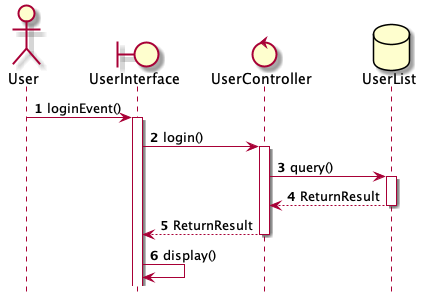
\includegraphics[width=12cm]{report/figure/sequenceDiagram/sd_login.png}
		    \caption{用户登录用例工作时序图}
		    \label{fig:sd_login}
		    %\end{adjustwidth}
		\end{figure}
	\end{enumerate}
	
	% subsection subsection_用户登录用例分析 (end)

% 	\subsection{发布母订单用例分析} % (fold)
% 	\label{sub:发布母订单用例分析}
% 	\begin{enumerate}
% 		\item \textbf{类的析取} \\
% 		发布母订单用例允许采购商进行母订单发布,其中包括的实体类、控制类和边界类如下图。
% 		\autoref{fig:class_apply}
% 		\begin{figure}[htp]
% 		    %\begin{adjustwidth}{-1.5cm}{-1cm}
% 		    \centering
% 		    
\includegraphics[width=12cm]{misc/figure_src/class_diagram/apply.png}
% 		    \caption{登录用例析取图}
% 		    \label{fig:class_apply}
% 		    %\end{adjustwidth}
% 		\end{figure}

% 		\item \textbf{用例工作时序图} \\ 
% 		发布母订单用例需要采购商登录后,点击发起母订单按钮,填写母订单信息后通过前端发送给后端,后端进行数据库操作后返回结果,正确的返回信息为待审核,具体流程如下图所示\autoref{fig:sd_generate}。

% 		\begin{figure}[htp]
% 		    %\begin{adjustwidth}{-1.5cm}{-1cm}
% 		    \centering
% 		    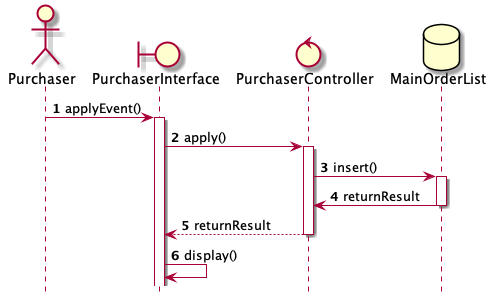
\includegraphics[width=12cm]{misc/figure_src/sequence_diagram/sd_applyMainOrder.png}
% 		    \caption{用户注册用例时序图}
% 		    \label{fig:sd_generate}
% 		    %\end{adjustwidth}
% 		\end{figure}

% 	\end{enumerate}
% 	% subsection 发布母订单用例分析 (end)
    \newpage
	\subsection{查看母订单用例分析} % (fold)
	\label{sub:查看母订单用例分析}
	\begin{enumerate}
		\item \textbf{类的析取} \\
		登录用例允许管理员、微供应商和采购商这三个类型的用户进行母订单相关查询,其中包括的实体类、控制类和边界类如下图
		\autoref{fig:class_queryMainOrder}。
		\begin{figure}[htp]
		    %\begin{adjustwidth}{-1.5cm}{-1cm}
		    \centering
		    
\includegraphics[width=12cm]{report/figure/classAnalyse/queryMainOrder.png}
		    \caption{查看母订单用例析取图}
		    \label{fig:class_queryMainOrder}
		    %\end{adjustwidth}
		\end{figure}

		\item \textbf{用例工作时序图} \\
		查看母订单用例需要用户登录后,在端点击“母订单查询”并填写相应信息后,将查询信息发送到后端,在后端进行数据库操作后返回结果,具体流程如下图所示\autoref{fig:sd_queryMainOrder}。

		\begin{figure}[htp]
		    %\begin{adjustwidth}{-1.5cm}{-1cm}
		    \centering
		    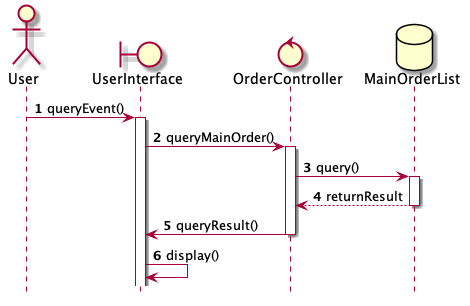
\includegraphics[width=12cm]{report/figure/sequenceDiagram/sd_queryMainOrder.png}
		    \caption{查看母订单用例工作时序图}
		    \label{fig:sd_queryMainOrder}
		    %\end{adjustwidth}
		\end{figure}

	\end{enumerate}
	
	% subsection 查看母订单用例分析 (end)

% 	\subsection{提交子订单用例分析} % (fold)
% 	\label{sub:提交子订单用例分析}
% 	\begin{enumerate}
% 		\item \textbf{类的析取} \\
% 		提交子订单用例允许微供应商在加入某个母订单并且通过审查后在相应子订单上更新自己的完成进度,其中包括的实体类、控制类和边界类如下图。
% 		\autoref{fig:class_commit}
% 		\begin{figure}[htp]
% 		    %\begin{adjustwidth}{-1.5cm}{-1cm}
% 		    \centering
% 		    
\includegraphics[width=12cm]{misc/figure_src/class_diagram/commit.png}
% 		    \caption{登录用例析取图}
% 		    \label{fig:class_commit}
% 		    %\end{adjustwidth}
% 		\end{figure}

% 		\item \textbf{用例工作时序图} \\
% 		在提交子订单用例中,微供应商填写进度信息等更新信息,由前端发送到后端,再在后端进行数据暂存等待管理员审核后返回相应的执行结果。具体流程如下图所示\autoref{fig:sd_commit}。

% 		\begin{figure}[htp]
% 		    %\begin{adjustwidth}{-1.5cm}{-1cm}
% 		    \centering
% 		    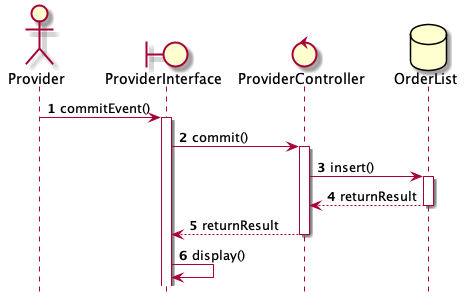
\includegraphics[width=12cm]{misc/figure_src/sequence_diagram/sd_commitOrder.png}
% 		    \caption{用户注册用例时序图}
% 		    \label{fig:sd_commit}
% 		    %\end{adjustwidth}
% 		\end{figure}

% 	\end{enumerate}
% 	% subsection 提交子订单用例分析 (end)

    \newpage
	\subsection{查看子订单用例分析} % (fold)
	\label{sub:查看子订单用例分析}
	\begin{enumerate}
		\item \textbf{类的析取} \\
		查看子订单用例允许管理员、微供应商和采购商在各自权限下查询子订单,其中包括的实体类、控制类和边界类如下图\autoref{fig:class_commit}。
		\begin{figure}[htp]
		    %\begin{adjustwidth}{-1.5cm}{-1cm}
		    \centering
		    
\includegraphics[width=12cm]{report/figure/classAnalyse/querySubOrder.png}
		    \caption{查看子订例析取图}
		    \label{fig:class_commit}
		    %\end{adjustwidth}
		\end{figure}

		\item \textbf{查看子订用例工作时序图} \\
		在查看子订单用例中,用户在前端填写查询信息,由端发送到后端,后端进行数据库操作后得到结果返回前端。具体流程如下图所示\autoref{fig:sd_querySubOrder}。

		\begin{figure}[htp]
		    %\begin{adjustwidth}{-1.5cm}{-1cm}
		    \centering
		    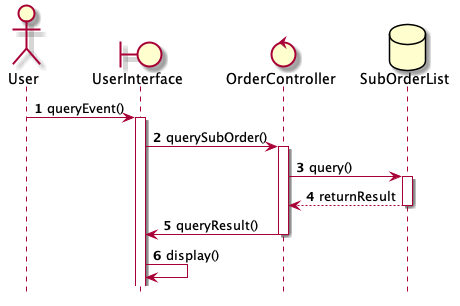
\includegraphics[width=12cm]{report/figure/sequenceDiagram/sd_querySubOrder.png}
		    \caption{查看子订用例工作时序图}
		    \label{fig:sd_querySubOrder}
		    %\end{adjustwidth}
		\end{figure}
	\end{enumerate}
	
	% subsection 查看子订单用例分析 (end)

% 	\subsection{用户查询用例分析} % (fold)
% 	\label{sub:用户查询用例分析}
% 	\begin{enumerate}
% 		\item \textbf{类的析取} \\
% 		用户查询用例允许管理员查询用户信息,其中包括的实体类、控制类和边界类如下图。
% 		% \autoref{fig:class_auditUser}
% 		% \begin{figure}[htp]
% 		%     %\begin{adjustwidth}{-1.5cm}{-1cm}
% 		%     \centering
% 		%     
\includegraphics[width=12cm]{misc/figure_src/class_diagram/auditUser.png}
% 		%     \caption{登录用例析取图}
% 		%     \label{fig:class_auditUser}
% 		%     %\end{adjustwidth}
% 		% \end{figure}

% 		\item \textbf{用例工作时序图} \\
% 		在用户查询用例中,管理员可以在前端填写查询信息后点击查询,该查询信息由前端发送到后端,后端进行数据库操作后得到结果返回前端。具体流程如下图所示\autoref{fig:sd_auditUser}。

% 		% \begin{figure}[htp]
% 		%     %\begin{adjustwidth}{-1.5cm}{-1cm}
% 		%     \centering
% 		%     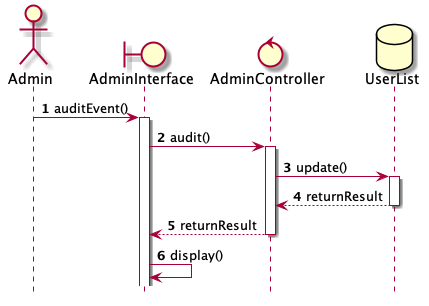
\includegraphics[width=12cm]{misc/figure_src/sequence_diagram/sd_audit_user.png}
% 		%     \caption{用户注册用例时序图}
% 		%     \label{fig:sd_auditUser}
% 		%     %\end{adjustwidth}
% 		% \end{figure}

% 	\end{enumerate}
% 	% subsection 用户查询用例分析 (end)

% 	\subsection{用户管理用例分析} % (fold)
% 	\label{sub:用户审核用例分析}
% 	\begin{enumerate}
% 		\item \textbf{类的析取} \\
% 		用户审核用例允许管理员处理微供应商和采购商提交的注册信息,管理员可以执行审核通过和审核不通过两种操作,其中包括的实体类、控制类和边界类如下图。
% 		\autoref{fig:class_auditUser}
% 		\begin{figure}[htp]
% 		    %\begin{adjustwidth}{-1.5cm}{-1cm}
% 		    \centering
% 		    
\includegraphics[width=12cm]{misc/figure_src/class_diagram/auditUser.png}
% 		    \caption{登录用例析取图}
% 		    \label{fig:class_auditUser}
% 		    %\end{adjustwidth}
% 		\end{figure}

% 		\item \textbf{用例工作时序图} \\
% 		在用户审核用例中,管理员在已经进行用户查询找到待审核用户后,可以在前端点击通过审核,审核确认信息由前端发送到后端,后端进行数据库操作后得到结果返回前端。具体流程如下图所示\autoref{fig:sd_auditUser}。

% 		\begin{figure}[htp]
% 		    %\begin{adjustwidth}{-1.5cm}{-1cm}
% 		    \centering
% 		    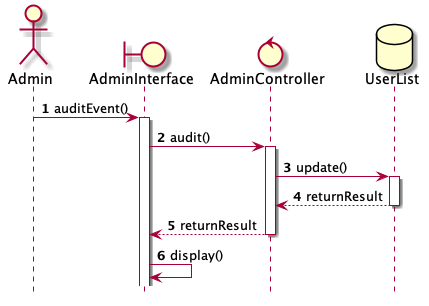
\includegraphics[width=12cm]{misc/figure_src/sequence_diagram/sd_audit_user.png}
% 		    \caption{用户管理用例时序图}
% 		    \label{fig:sd_auditUser}
% 		    %\end{adjustwidth}
% 		\end{figure}

% 	\end{enumerate}
% 	% subsection 用户审核用例分析 (end)

% 	\subsection{订单审核用例分析} % (fold)
% 	\label{sub:订单审核用例分析}
% 	\begin{enumerate}
% 		\item \textbf{类的析取} \\
% 		订单审核用例允许管理员审核来自采购商的订单申请和微供应商的更新子订单进度的申请,其中包括的实体类、控制类和边界类如下图。
% 		\autoref{fig:class_auditOrder}
% 		\begin{figure}[htp]
% 		    %\begin{adjustwidth}{-1.5cm}{-1cm}
% 		    \centering
% 		    
\includegraphics[width=12cm]{misc/figure_src/class_diagram/auditOrder.png}
% 		    \caption{登录用例析取图}
% 		    \label{fig:class_auditOrder}
% 		    %\end{adjustwidth}
% 		\end{figure}

% 		\item \textbf{用例工作时序图} \\
% 		在用户审核用例中,管理员在已经进行订单查询找到待审核用户后,可以在前端点击通过审核,审核确认信息由前端发送到后端,后端进行数据库操作后得到结果返回前端。具体流程如下图所示\autoref{fig:sd_auditOrder}

% 		\begin{figure}[htp]
% 		    %\begin{adjustwidth}{-1.5cm}{-1cm}
% 		    \centering
% 		    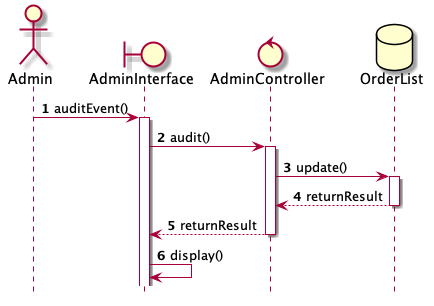
\includegraphics[width=12cm]{misc/figure_src/sequence_diagram/sd_audit_order.png}
% 		    \caption{用户注册用例时序图}
% 		    \label{fig:sd_auditOrder}
% 		    %\end{adjustwidth}
% 		\end{figure}
% 	\end{enumerate}

\newpage
	\subsection{订单加入用例分析} % (fold)
	\label{sub:订单加入用例分析}
	\begin{enumerate}
		\item \textbf{类的析取} \\
		订单加入用例允许微供应商在查询了母订单后加入某母订单,并在数据库中生成对应的子订单信息,其中包括的实体类、控制类和边界类如下图
		\autoref{fig:class_join}。
		\begin{figure}[htp]
		    %\begin{adjustwidth}{-1.5cm}{-1cm}
		    \centering
		    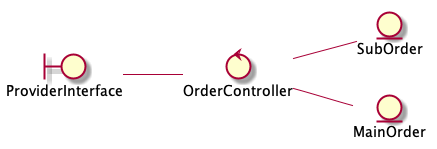
\includegraphics[width=12cm]{report/figure/classAnalyse/join.png}
		    \caption{订单加入用例析取图}
		    \label{fig:class_join}
		    %\end{adjustwidth}
		\end{figure}

		\item \textbf{用例工作时序图} \\
		在订单加入用例中,微供应商在已经查询了母订单信息后可以选择合适的母订单加入,在前端点击“加入”后,该信息发送到后端并生成子订单信息并修改母订单。具体流程如下图所示\autoref{fig:sd_joinOrder}

		\begin{figure}[htp]
		    %\begin{adjustwidth}{-1.5cm}{-1cm}
		    \centering
		    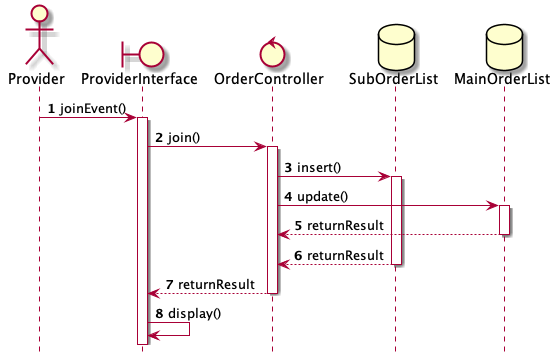
\includegraphics[width=12cm]{report/figure/sequenceDiagram/sd_joinOrder.png}
		    \caption{订单加入用例工作时序图}
		    \label{fig:sd_joinOrder}
		    %\end{adjustwidth}
		\end{figure}
	\end{enumerate}
	
	% subsection 订单加入用例分析 (end)

\section{分析机制} 
	根据 1.4 补充规约得到上述边界类、控制类、实体类需要满足的非功能性需求, 列出系统的分析机制表,如下表所示:

	\begin{table}[h]
		\centering
		\caption{”鲜天下“平台分析机制}
		\begin{tabular}{|c|c|}
			\hline  
				分析类 & 分析机制性\\
			\hline  
				User & 持久性、安全性\\
			\hline  
				MainOrder & 持久性、安全性\\
			\hline
				SubOrder & 持久性、安全性\\
			\hline  
				UserInterface & 持久性、遗留接口\\
			\hline
				UserController & 分布式\\
			\hline
		\end{tabular}
	\end{table}



\section{合并分析类}

% TODO: 类图

	将析取出来的边界类、控制类、实体类进行合并整理,得到的系统的合并类图如下图所示:\\
	\begin{figure}[htp]
		    \begin{adjustwidth}{-1cm}{-1cm}
		    \centering
		    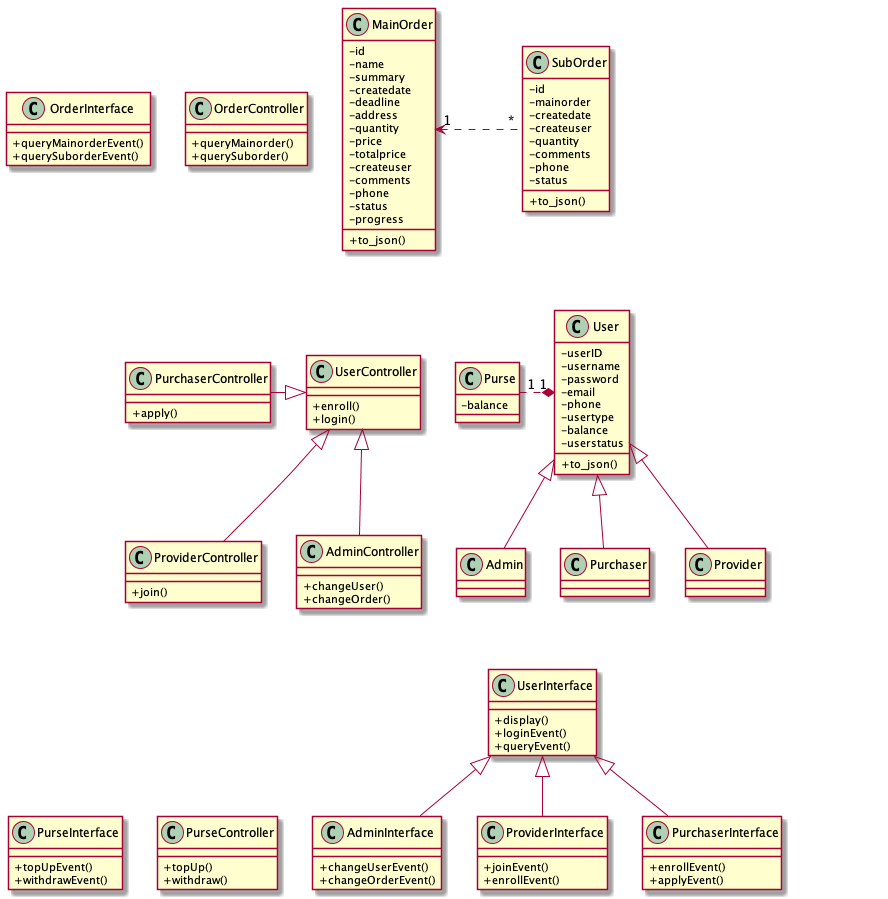
\includegraphics[width=20cm]{report/figure/class_system.png}
		    \caption{“鲜天下”平台合并类图}
		    % \label{fig:class_join}
		    \end{adjustwidth}
		\end{figure}

        \newclearpage
        %% chapter 4 dataset, network structure, experiment and result
\chapter{实验与结果}
\label{cha:experiment}


        \newclearpage
        %%%%%%%%%%%%%%%%%%%%%%% 部件设计 %%%%%%%%%%%%%%%%%%%%%%%%%%%%%%%%%%%%%%%%%%%%%
\chapter{部件设计}

\section{分析并发需求}

在“鲜天下”系统中,并发性的要求来自于用户的需求。后端的实现若是串行的,后端暴露给前端的API可能会由于用户请求数的增加而导致请求延时增加,服务质量下降。由此,无论是相同的API被多个用户同时调用,还是不同的API被同时调用,都需要通过并发来降低请求延时,提升用户体验。

\section{识别相应的进程和线程}

\begin{enumerate}
    \item \textbf{多用户使用同一个服务}\\以查询母订单服务为例,下图描述了三个用户同时使用母订单查询功能时,“鲜天下”平台创建进程和线程来满足用户服务的过程。
    
    \begin{figure}[htp]
        %\begin{adjustwidth}{-1.5cm}{-1cm}
        \centering
        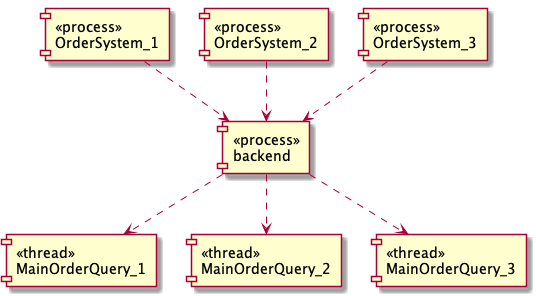
\includegraphics[width=12cm]{report/figure/component/query.png}
        \caption{多用户同时查询母订单的过程}
        \label{fig:query}
        %\end{adjustwidth}
    \end{figure}
    
    当多个用户同时进行母订单查询时,后台服务器会为每个用户的请求创建一个线程,当线程执行完查询操作时,会各自返回其结果。
    
    
    \item \textbf{多用户使用不同的服务}\\以查询子订单和查询母订单服务为例, 下图描述了两个用户分别使用查询子订单和查询母订单服务时,“鲜天下”平台创建进程和线程来满足用户服务的过程。
    \begin{figure}[htp]
        %\begin{adjustwidth}{-1.5cm}{-1cm}
        \centering
        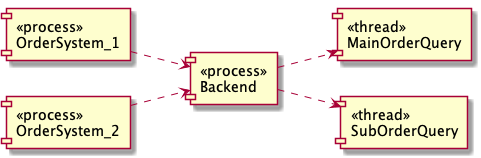
\includegraphics[width=12cm]{report/figure/component/process.png}
        \caption{多用户同时查询母订单的过程}
        \label{fig:query}
        %\end{adjustwidth}
    \end{figure}
    
    \newpage
    当多个用户同时请求不同的服务时,后台服务器会为每个用户的每个请求创建一个线程,线程执行完各自的操作后自动返回。
    
\end{enumerate}

\section{生命周期}

    如\autoref{fig:lifetime}所示,在多个用户同时调用相同(或不同)API的时候,后台会产生多个线程同时处理请求并返回相应的数据。

    \begin{figure}[htp]
        %\begin{adjustwidth}{-1.5cm}{-1cm}
        \centering
        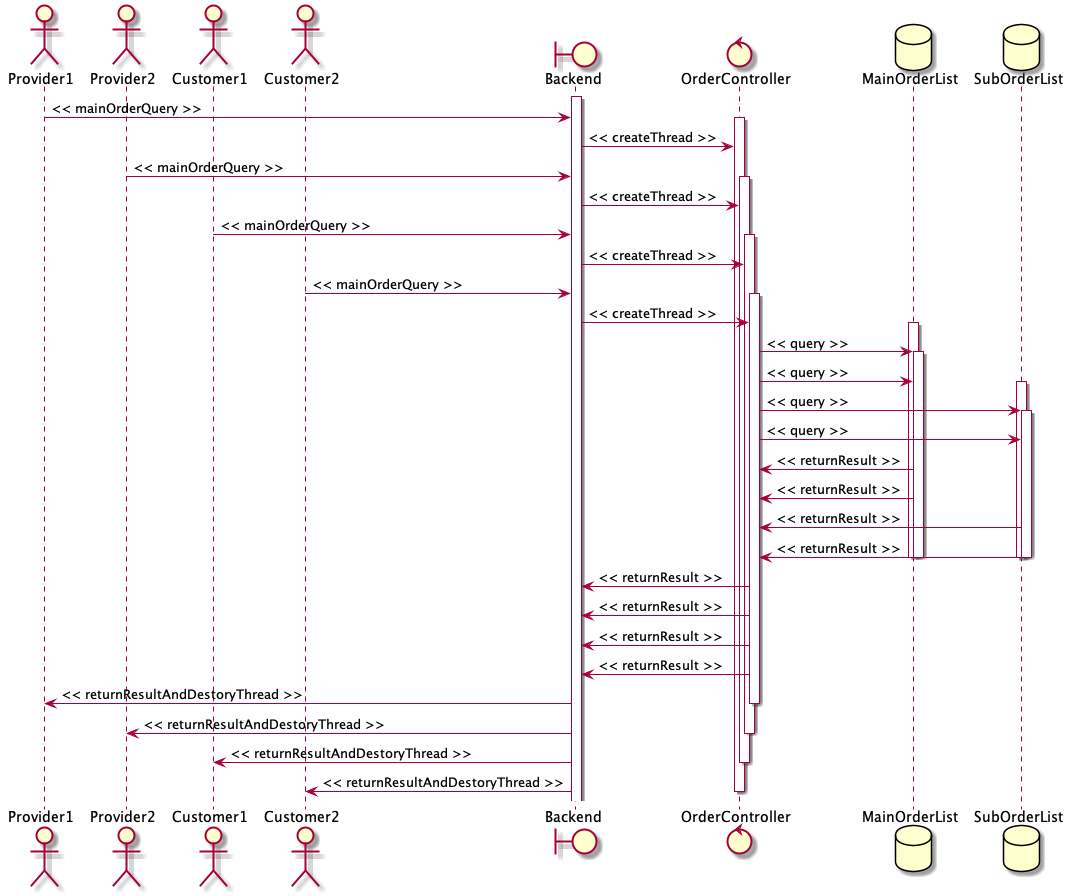
\includegraphics[width=15.5cm]{report/figure/component/lifetime.png}
        \caption{线程生命周期示意图}
        \label{fig:lifetime}
        %\end{adjustwidth}
    \end{figure}



\section{映射到现实系统}

我们的后端部署在CPU为Intel I7-7700,内存为16GB的服务器上,该CPU具备4个物理核心,8个逻辑核心,最大支持8个硬件线程。因此,后端的并发处理能够更好地利用处理器的性能,提升用户体验。
        \newclearpage
        % \chapter{简单的使用例子}
\label{cha:example}
\section{图像的插入}
\subsection{镶嵌在文中的图像}
\label{sec:Images}
\begin{wrapfigure}{r}{0.5\linewidth}
	\centering
	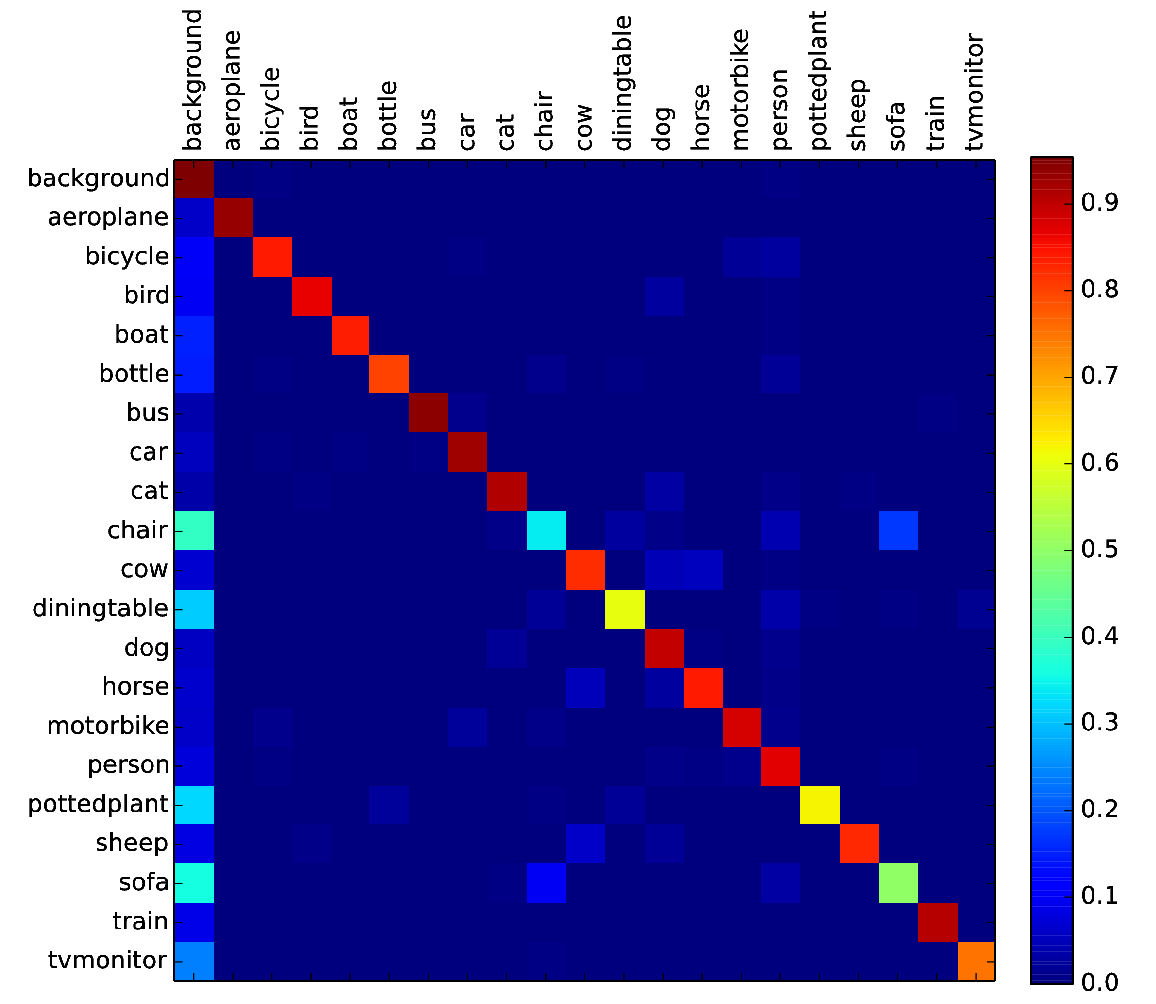
\includegraphics[width=0.5\textwidth]{image/result/confusion.pdf}
	\caption{镶嵌在文中的图像}
	\label{fig:confusion}
\end{wrapfigure}
论文主体是毕业论文的主要部分,必须言之成理,论据可靠,严格遵循本学科国际通行的学术规范。在写作上要注意结构合理、层次分明、重点突出,章节标题、公式图表符号必须规范统一。论文主体的内容根据不同学科有不同的特点,一般应包括以下几个方面: (1)毕业论文(设计)总体方案或选题的论证; (2)毕业论文(设计)各部分的设计实现,包括实验数据的获取、数据可行性及有效性的处理与分析、各部分的设计计算等; (3)对研究内容及成果的客观阐述,包括理论依据、创新见解、创造性成果及其改进与实际应用价值等; (4)论文主体的所有数据必须真实可靠,凡引用他人观点、方案、资料、数据等,无论曾否发表,无论是纸质或电子版,均应详加注释。自然科学论文应推理正确、结论清晰;人文和社会学科的论文应把握论点正确、论证充分、论据可靠,恰当运用系统分析和比较研究的方法进行模型或方案设计,注重实证研究和案例分析,根据分析结果提出建议和改进措施等。
\subsection{单张图像的插入}

\begin{figure}[h]
	\centering
	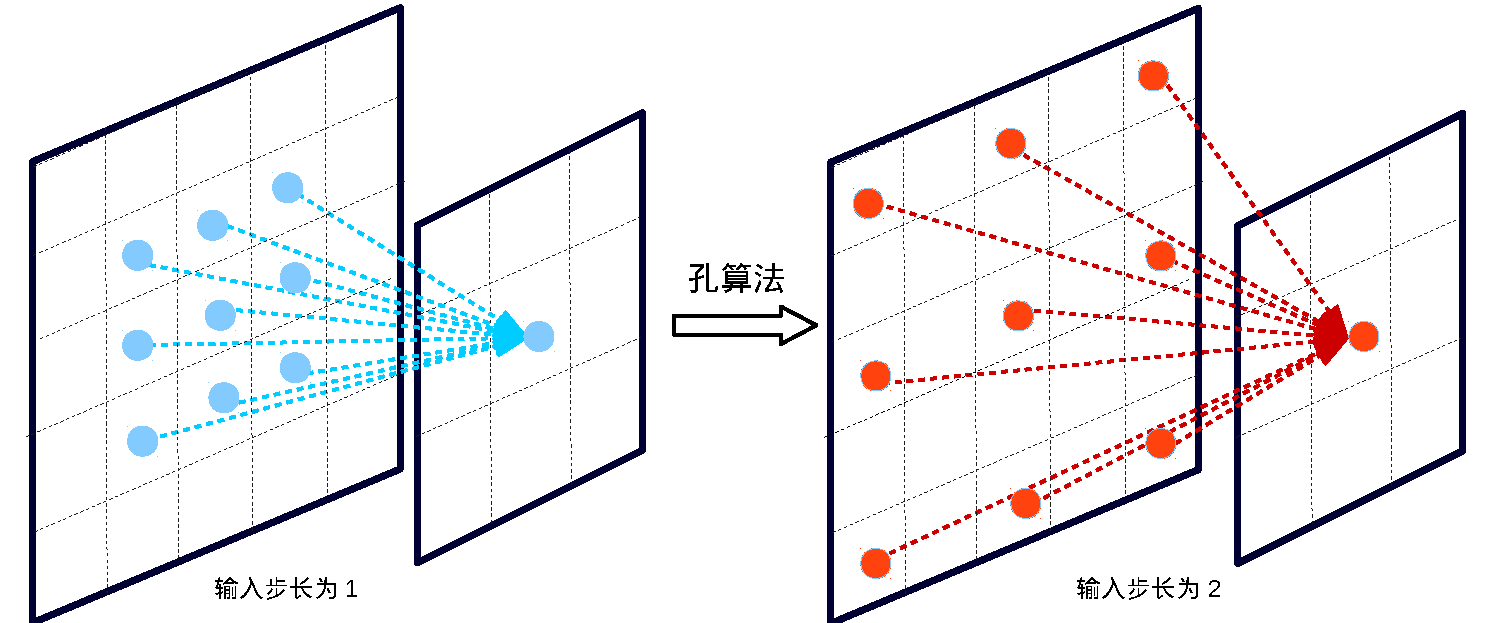
\includegraphics[width=0.5\textwidth]{image/illustration/hole.pdf}
	\caption{单张图像}
 	\label{fig:hole}
\end{figure}


\subsection{多张图像的并排插入}
\label{sub:多张图像的并排插入}


\begin{figure}[h!]%文中的Grid-LSTM模型做的语义图像分割的例子
	\centering
	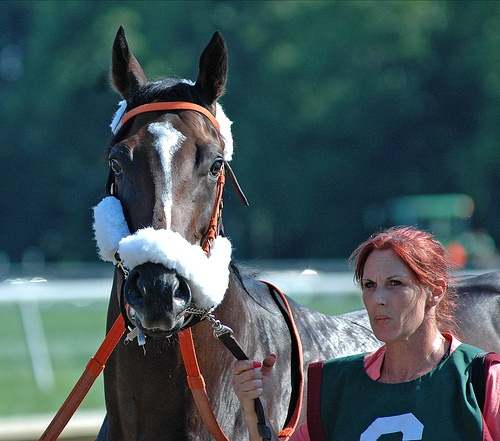
\includegraphics[width=.2\textwidth,height=.15\textwidth]{image/example/2007_000799.jpg}
	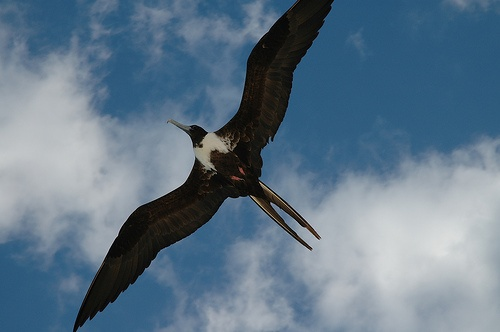
\includegraphics[width=.2\textwidth,height=.15\textwidth]{image/example/2007_002094.jpg}
	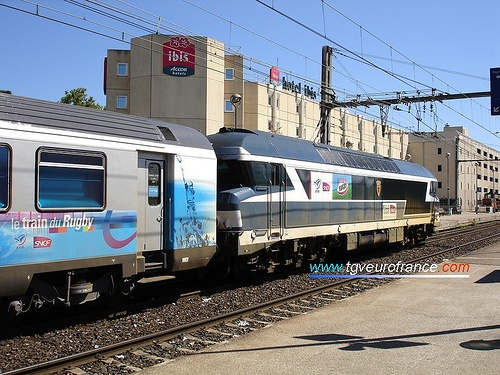
\includegraphics[width=.2\textwidth,height=.15\textwidth]{image/example/2007_004483.jpg}
	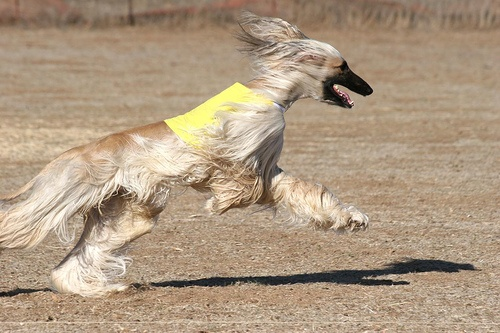
\includegraphics[width=.2\textwidth,height=.15\textwidth]{image/example/2007_003194.jpg}
	\\
	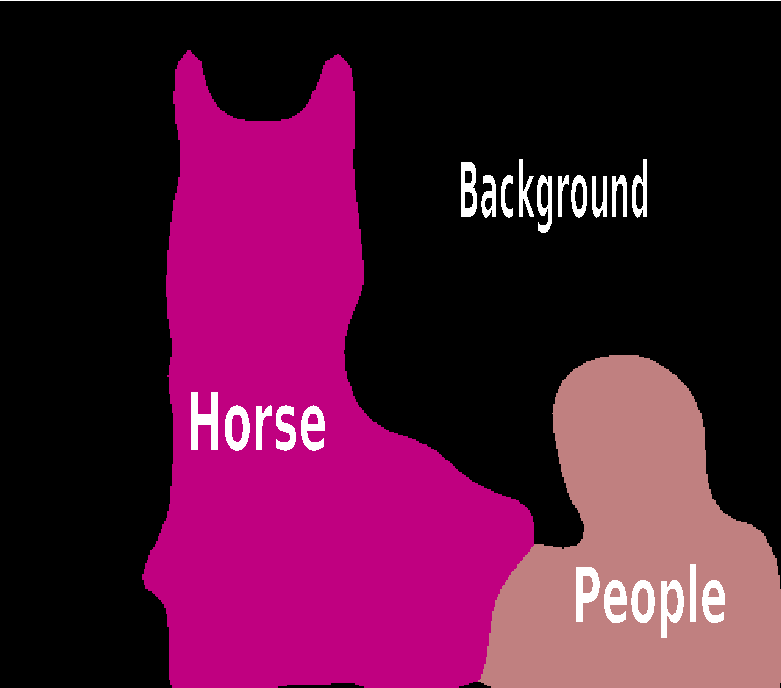
\includegraphics[width=.2\textwidth,height=.15\textwidth]{image/example/2007_000799.pdf}
	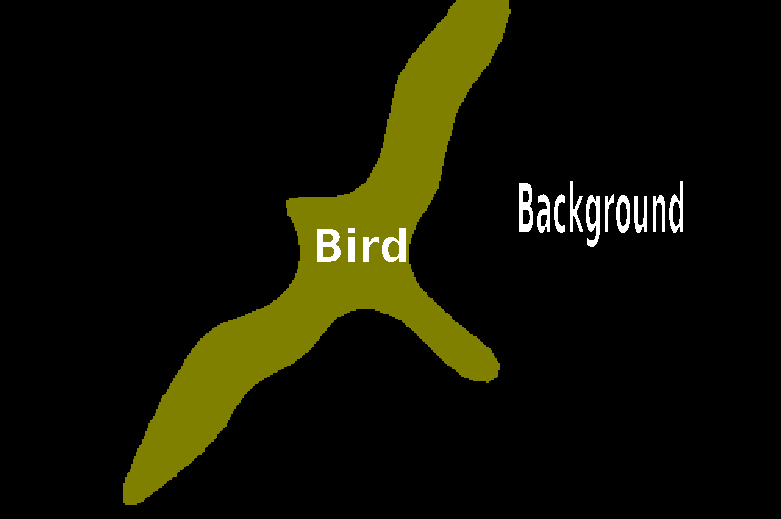
\includegraphics[width=.2\textwidth,height=.15\textwidth]{image/example/2007_002094.pdf}
	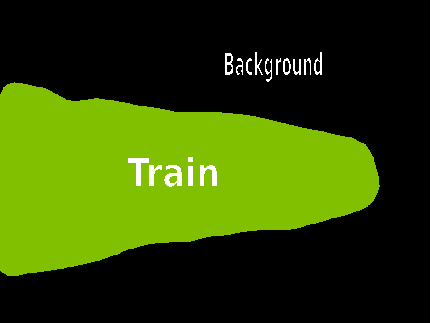
\includegraphics[width=.2\textwidth,height=.15\textwidth]{image/example/2007_004483.pdf}
	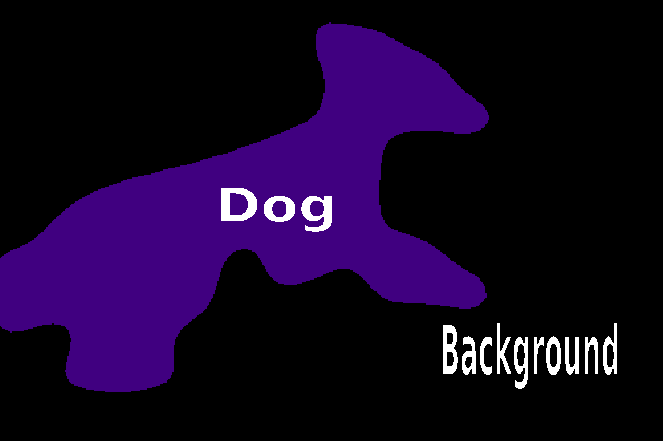
\includegraphics[width=.2\textwidth,height=.15\textwidth]{image/example/2007_003194.pdf}
	\caption{并排的多张图像}
	\label{fig:example1}
\end{figure}

\begin{figure}[h]
	\centering
		\makebox[0.11\textwidth]{\scriptsize 图像}
		\enspace
		\makebox[0.11\textwidth]{\scriptsize 真值}
		\enspace
		\makebox[0.11\textwidth]{\scriptsize CNN+5LSTM\textbf{1}}
		\enspace\thinspace
		\makebox[0.11\textwidth]{\scriptsize CNN+5LSTM\textbf{2}}
		\enspace\thinspace
		\makebox[0.11\textwidth]{\scriptsize CNN+5LSTM\textbf{3}}
		\enspace\thinspace
		\makebox[0.11\textwidth]{\scriptsize CNN+5LSTM\textbf{4}}
		\enspace\thinspace
		\makebox[0.11\textwidth]{\scriptsize CNN+5LSTM\textbf{5}}\\
		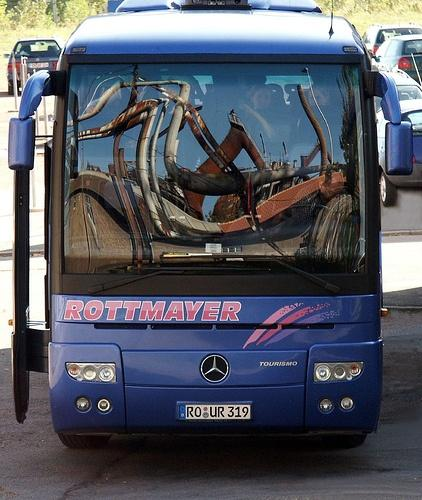
\includegraphics[width=0.11\textwidth]{image/improvement/2007_000663.jpg}
		\enspace\thinspace %\hfill
		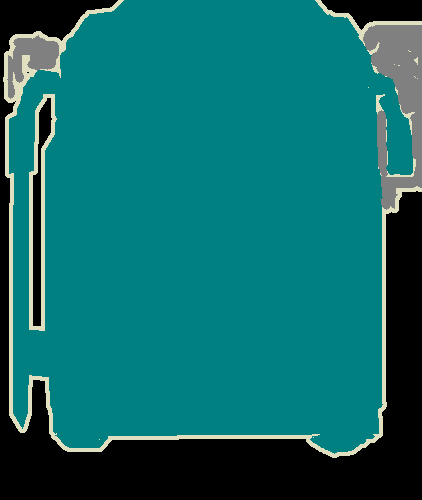
\includegraphics[width=0.11\textwidth]{image/improvement/2007_000663.png}
		\enspace\thinspace
		
\includegraphics[width=0.11\textwidth]{image/improvement/2007_000663_1.png}
		\enspace\thinspace
		
\includegraphics[width=0.11\textwidth]{image/improvement/2007_000663_2.png}
		\enspace\thinspace
		
\includegraphics[width=0.11\textwidth]{image/improvement/2007_000663_3.png}
		\enspace\thinspace
		
\includegraphics[width=0.11\textwidth]{image/improvement/2007_000663_4.png}
		\enspace\thinspace
		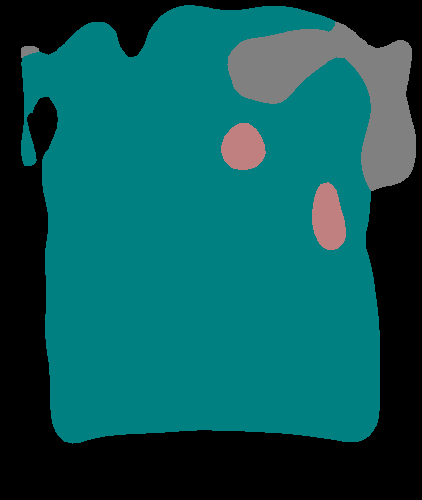
\includegraphics[width=0.11\textwidth]{image/improvement/2007_000663_5.png}
		\enspace\thinspace
		\caption{并排的多张图像加各自的注解}
		\label{fig:improvement}
	\end{figure}
	

\subsection{两列图像的插入}
\label{sec:complex}

\begin{figure}[h!] % image examples & compare
	\begin{subfigure}{0.55\textwidth}
		\makebox[0.18\textwidth]{\scriptsize Grid-5LSTM}
		\makebox[0.18\textwidth]{\scriptsize FCN-8s\cite{long2015fully}}
		\makebox[0.18\textwidth]{\scriptsize SDS\cite{hariharan2014simultaneous}}
		\makebox[0.18\textwidth]{\scriptsize 真值}
		\makebox[0.18\textwidth]{\scriptsize 图像} \\
		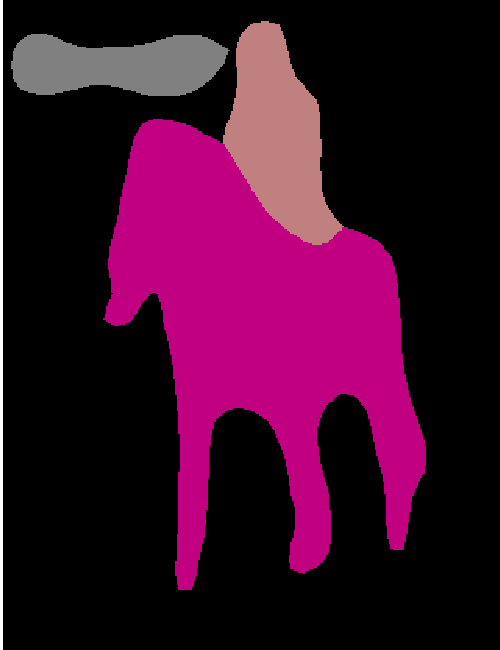
\includegraphics[width=0.18\textwidth]{image/result/compare/my_horse.pdf}
		
\includegraphics[width=0.18\textwidth]{image/result/compare/fcn_horse.png}
		
\includegraphics[width=0.18\textwidth]{image/result/compare/sds_horse.png}
		
\includegraphics[width=0.18\textwidth]{image/result/compare/gt_horse.pdf}
		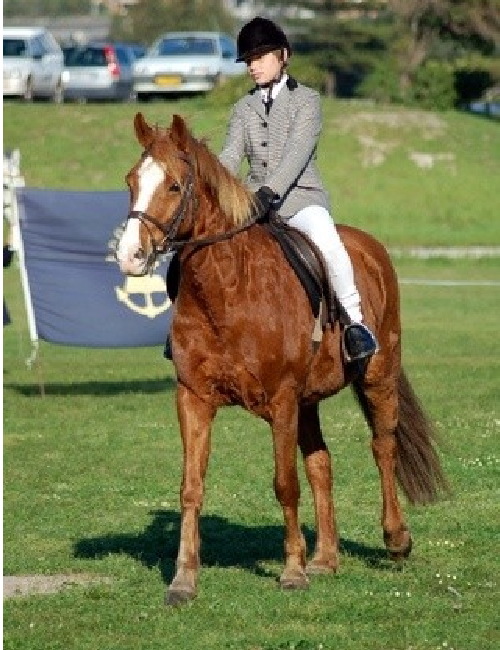
\includegraphics[width=0.18\textwidth]{image/result/compare/im_horse.pdf}
		\\
		
\includegraphics[width=0.18\textwidth]{image/result/compare/my_motor.png}
		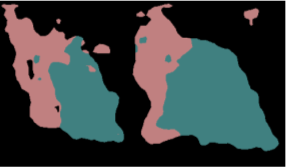
\includegraphics[width=0.18\textwidth]{image/result/compare/fcn_motor.png}
		
\includegraphics[width=0.18\textwidth]{image/result/compare/sds_motor.png}
		
\includegraphics[width=0.18\textwidth]{image/result/compare/2007_005173.png}
		\includegraphics[width=0.18\textwidth]{image/result/compare/2007_005173.jpg}
		\\
		\includegraphics[width=0.18\textwidth]{image/result/compare/my_sheep.pdf}
		\includegraphics[width=0.18\textwidth]{image/result/compare/fcn_sheep.png}
		\includegraphics[width=0.18\textwidth]{image/result/compare/sds_sheep.png}
		\includegraphics[width=0.18\textwidth]{image/result/compare/gt_sheep.pdf}
		\includegraphics[width=0.18\textwidth]{image/result/compare/im_sheep.pdf}
		\\
		\includegraphics[width=0.18\textwidth]{image/result/compare/my_boat.png}
		\includegraphics[width=0.18\textwidth]{image/result/compare/fcn_boat.png}
		\includegraphics[width=0.18\textwidth]{image/result/compare/sds_boat.png}
		\includegraphics[width=0.18\textwidth]{image/result/compare/2007_004241.png}
		\includegraphics[width=0.18\textwidth]{image/result/compare/2007_004241.jpg}
		\caption{左边的图像}
		\label{fig:compare1}
	\end{subfigure}
	\begin{subfigure}{0.4\textwidth}
		\centering
%		\makebox[0.3\textwidth]{} \\
%		\makebox[0.3\textwidth]{} \\
		\includegraphics[width=0.25\textwidth]{image/result/compare/2010_005284.jpg}
		\includegraphics[width=0.25\textwidth]{image/result/compare/2007_003349.jpg}
		\includegraphics[width=0.25\textwidth]{image/result/compare/2009_004507.jpg} 
		\\
		\includegraphics[width=0.25\textwidth]{image/result/compare/2010_005284.png}
		\includegraphics[width=0.25\textwidth]{image/result/compare/2007_003349.png}
		\includegraphics[width=0.25\textwidth]{image/result/compare/2009_004507.png} \\
		\includegraphics[width=0.25\textwidth]{image/result/compare/zoom_bus.png}
		\includegraphics[width=0.25\textwidth]{image/result/compare/zoom_bird.png}
		\includegraphics[width=0.25\textwidth]{image/result/compare/zoom_dog.png} \\
		\includegraphics[width=0.25\textwidth]{image/result/compare/deeplab_bus.png}
		\includegraphics[width=0.25\textwidth]{image/result/compare/deeplab_bird.png}
		\includegraphics[width=0.25\textwidth]{image/result/compare/deeplab_dog.png} \\
		\includegraphics[width=0.25\textwidth]{image/result/compare/my_bus.png}
		\includegraphics[width=0.25\textwidth]{image/result/compare/my_bird.png}
		\includegraphics[width=0.25\textwidth]{image/result/compare/my_dog.png} 
		\caption{右边的图像}
		\label{fig:compare2}
	\end{subfigure}
	\caption{复杂的两列对象的插入}
	\label{fig:complex}
\end{figure}



\clearpage

\section{表格的插入}
\label{sec:tables}


\begin{table}[h] %voc table result
	\centering
		\begin{tabular}{*{4}{c}}
			\toprule
	 		Method & Pixel Acc. & Mean Acc. & Mean Iu.\\
			\midrule
			Liu等人\cite{liu2011sift}  & 76.7 & - & -\\
		Tighe等人\cite{tighe2013finding}  & 78.6 & 39.2 & -\\
			FCN-16s\cite{long2015fully} & 85.2 & \textbf{51.7} & 39.5\\
			Deeplab-LargeFOV\cite{chen14semantic} & 85.6 & 51.2 & 39.7\\
			\midrule
			Grid-LSTM5 & \textbf{86.2} & 51.0 & \textbf{41.2}\\
			\bottomrule
		\end{tabular}
		\caption{典型的实验对比表格}		
		\label{tab:siftflow}
\end{table}


\begin{table}[h] %voc table result
	\centering
		\resizebox{\textwidth}{!}{
		\begin{tabular}{c|*{20}{c}|c}
			\toprule
			Method & aero & bike & bird & boat & bottle & bus & car & cat & chair & cow & table & dog & horse & mbike & person & plant & shep & sofa & train & tv & mIoU.\\
			\midrule
			CNN				   & 72.6 & 29.6 & 70.2 & 53.1 & 65.1 & 81.0 & 74.3 & 79.8 & 25.0 & 64.8 & 47.8 & 69.5 & 66.2 & 65.2 & 74.2 & 42.1 & 69.6 & 38.8 & 74.4 & 58.6 & 62.5\\
			CNN+\textbf{1}LSTM & 71.5 & 30.6 & 70.5 & 53.8 & 64.9 & 82.4 & 77.1 & 79.5 & 25.1 & 65.8 & 47.8 & 71.5 & 64.6 & 67.0 & 74.0 & 43.9 & 69.6 & 38.6 & 74.9 & 59.4 & 63.0\\
			CNN+\textbf{2}LSTM & 76.1 & 32.6 & 72.1 & 57.0 & 65.3 & 83.6 & 75.4 & 81.7 & 24.7 & 69.3 & 47.5 & 72.3 & 68.9 & 69.5 & 74.7 & 41.5 & 69.8 & 38.3 & 77.8 & 62.1 & 64.3 \\
			CNN+\textbf{3}LSTM & 77.7 & 32.3 & 72.6 & 60.0 & 68.3 & 85.5 & 78.5 & 82.3 & 25.3 & 71.1 & 49.7 & 71.5 & 69.7 & 70.8 & 75.9 & 47.9 & 71.2 & 38.9 & 80.2 & 61.7 & 65.8 \\
			CNN+\textbf{4}LSTM & 79.1 & \textbf{33.7} & \textbf{73.6} & \textbf{62.0} & \textbf{70.4} & 85.5 & \textbf{80.9} & 83.7 & \textbf{24.1} & 70.7 & 45.7 & 73.7 & 69.6 & 72.1 & 75.6 & 47.2 & \textbf{76.0} & 37.3 & 80.5 & 62.2 & 66.4 \\
			CNN+\textbf{5}LSTM & \textbf{79.9} & 33.6 & \textbf{73.6} & 61.7 & 68.0 & \textbf{88.5} & \textbf{80.9} & \textbf{84.0} & 23.6 & \textbf{71.3} & \textbf{49.7} & \textbf{73.1} & \textbf{71.3} & \textbf{72.9} & \textbf{76.4} & \textbf{48.9} & 75.1 & \textbf{38.1} & \textbf{84.5} & \textbf{63.8} & \textbf{67.2} \\
			\midrule
			CNN+\textbf{5}LSTM$^\dag$ & 84.8 & 36.4 & 82.0 & 69.4 & 73.0 & 87.2 & 81.8 & 86.1 & 34.5 & 82.4 & 53.1 & 81.5 & 77.4 & 79.0 & 81.3 & 54.8 & 81.1 & 47.0 & 84.3 & 67.3 & 72.3 \\
			\bottomrule
		\end{tabular}}
		\caption{复杂一些的表格}		
		\label{tab:vocval}
	\end{table}
	

\section{公式}
\label{sec:formula}
没有编号的公式
\begin{align*}
\begin{split}
	\label{eq:feedforward}
	\mybold{z}^{(l)} & = \mybold{W}^{(l)}\mybold{a}^{(l-1)} + \mybold{b}^{(l)} \\
	\mybold{a}^{(l)} & = f(\mybold{z}^{(l)})
\end{split}
\end{align*}
公式中含有中文
\begin{align}
	\begin{split}
	\mbox{像素准确率} &= \sum_{i=1}^{n_{cl}}n_{ii} / \sum_{i=1}^{n_{cl}}t_i \\
		\mbox{平均像素准确率} &= \frac{1}{n_{cl}} \sum_{i=1}^{n_{cl}}(n_{ii}/ t_i) \\
	\mbox{Mean IU} &= \frac{1}{n_{cl}} \sum_{i=1}^{n_{cl}}\frac{n_{ii}}{t_i + \sum_j^{n_{cl}} n_{ji} - n_{ii}}
	\end{split}
\end{align}
公式中含有矩阵
\begin{equation}
	\textbf{H} = \begin{bmatrix}
		I*\mybold{x}_i \\ \textbf{h}
	\end{bmatrix}
\end{equation}
每行后面都有编号的公式
\begin{align}
	\frac{\partial}{\partial W_{ij}^{(l)}} J(\mybold{W},\mybold{b};\mybold{x},y) &= \frac{\partial J(\mybold{W},\mybold{b};\mybold{x},y)}{\partial z_i^{(l+1)}}\cdot \frac{\partial z_i^{(l+1)}}{\partial W_{ij}^{(l)}} = \delta_i^{(l+1)}a_j^{(l)} \\
	\frac{\partial}{\partial b_i^{(l)}} J(\mybold{W},\mybold{b};\mybold{x},y) &= \frac{\partial J(\mybold{W},\mybold{b};\mybold{x},y)}{\partial z_i^{(l+1)}}\cdot \frac{\partial z_i^{(l+1)}}{\partial b_i^{(l)}} = \delta_i^{(l+1)}
\end{align}

\section{算法流程图}
\label{sec:algorithm}
\begin{algorithm}[h]
\KwIn{$m$个训练样本}
\lFor{$l=1$ \emph{\KwTo} $n_l$}{
初始化:$\Delta \mybold{W}^{(l)}=0$,$\Delta \mybold{b}^{(l)}=0$}
\ForEach{训练样本}{
	\lFor{$l=1$ \emph{\KwTo} $n_l-1$}{
	前向传播:$\mybold{z}^{(l+1)}=\mybold{W}^la^l+\mybold{b}^l$,$\mybold{a}^{(l+1)}=f(\mybold{z}^{(l+1)})$}
	输出误差计算:$\delta^{(n_l)} = \frac{\partial}{\partial \mybold{z}^{(n_l)}} J(\mybold{W},\mybold{b};\mybold{x},y)$\;
	\lFor{$l=n_l-1$ \emph{\KwTo} $1$}{
	后向传播:$\delta^{(l)} = \bigl((\mybold{W}^{(l)})^T \delta^{(l+1)}\bigr)f'(\mybold{z}^{(l)})$}
	\ForAll{层l}{
		计算梯度:$\nabla_{\mybold{W}^{(l)}}J(\mybold{W},\mybold{b};\mybold{x},y)=\delta^{(l+1)}(\mybold{a}^{(l)})^T$ \\
		\hspace{60pt}$\nabla_{\mybold{b}^{(l)}}J(\mybold{W},\mybold{b};\mybold{x},y)=\delta^{(l+1)}$\;
		累加梯度:$\Delta \mybold{W}^{(l)} \leftarrow \Delta \mybold{W}^{(l)} + \nabla_{\mybold{W}^{(l)}}J(\mybold{W},\mybold{b};\mybold{x},y)$; \\
		\hspace{60pt}$\Delta \mybold{b}^{(l)} \leftarrow \Delta \mybold{b}^{(l)} + \nabla_{\mybold{b}^{(l)}}J(\mybold{W},\mybold{b};\mybold{x},y)$\;
	}
}
\ForAll{层$l$}{
	更新权重:$\mybold{W}^{(l)} \leftarrow \mybold{W}^{(l)} - \alpha \biggl[\frac 1m \Delta \mybold{W}^{(l)}]$ \\
	\hspace{60pt} $\mybold{b}^{(l)} \leftarrow \mybold{b}^{(l)} - \alpha \biggl[\frac 1m \Delta \mybold{b}^{(l)}\biggr]$
}
\caption{梯度下降算法}
\label{algo:sgd}
\end{algorithm}

\section{例子与证明}
\subsection{例子}
\begin{eg}
  这是一个例子, 用以验证特殊环境的字体成功更改为楷体.
\end{eg}

\begin{proof}

  1. 大前提 \\
  2. 小前提 \\
  结论: 示例结论 \\
\end{proof}

\section{其他的一些用法}
\label{sec:font}
\subsection{子章节编号}
\label{sec:font:subsection}
\subsubsection{更小的章节}
\label{sec:font:subsection:subsub}
更小的章节编号也是支持的。

\subsection{列表的使用}
\label{src:font:list}

这是一个无序列表
\begin{itemize}
	\item 引用文献\cite{long2015fully}
	\item 字体{\color{red}{变红}},\textbf{粗体}
\end{itemize}

这是一个有序列表
\begin{enumerate}
	\item 索引前面的章节 \ref{sec:formula}、图像\ref{fig:complex}、表格\ref{tab:siftflow}
	\item 加脚注\footnote{http://cs231n.github.io/transfer-learning/}
\end{enumerate}



\begin{figure}[h!]
	\centering
			\makebox[0.16\textwidth]{\scriptsize 图像}
			\makebox[0.16\textwidth]{\scriptsize 真值}
			\makebox[0.16\textwidth]{\scriptsize Grid-5LSTM1}
			\makebox[0.16\textwidth]{\scriptsize Grid-5LSTM3}
			\makebox[0.16\textwidth]{\scriptsize Grid-5LSTM5} \\
			\includegraphics[width=0.16\textwidth]{image/appendix1/2007_000042.jpg}
			\includegraphics[width=0.16\textwidth]{image/appendix1/2007_000042.png}
			\includegraphics[width=0.16\textwidth]{image/appendix1/1/2007_000042.png} 
			\includegraphics[width=0.16\textwidth]{image/appendix1/3/2007_000042.png}
			\includegraphics[width=0.16\textwidth]{image/appendix1/5/2007_000042.png} \\
	
			\includegraphics[width=0.16\textwidth]{image/appendix1/2011_003256.jpg}
			\includegraphics[width=0.16\textwidth]{image/appendix1/2011_003256.png}
			\includegraphics[width=0.16\textwidth]{image/appendix1/1/2011_003256.png} 
			\includegraphics[width=0.16\textwidth]{image/appendix1/3/2011_003256.png}
			\includegraphics[width=0.16\textwidth]{image/appendix1/5/2011_003256.png} \\
			\includegraphics[width=0.16\textwidth]{image/appendix1/2011_001159.jpg}
			\includegraphics[width=0.16\textwidth]{image/appendix1/2011_001159.png}
			\includegraphics[width=0.16\textwidth]{image/appendix1/1/2011_001159.png} 
			\includegraphics[width=0.16\textwidth]{image/appendix1/3/2011_001159.png}
			\includegraphics[width=0.16\textwidth]{image/appendix1/5/2011_001159.png} \\
			\includegraphics[width=0.16\textwidth]{image/appendix1/2011_000813.jpg}
			\includegraphics[width=0.16\textwidth]{image/appendix1/2011_000813.png}
			\includegraphics[width=0.16\textwidth]{image/appendix1/1/2011_000813.png} 
			\includegraphics[width=0.16\textwidth]{image/appendix1/3/2011_000813.png}
			\includegraphics[width=0.16\textwidth]{image/appendix1/5/2011_000813.png} \\
			\includegraphics[width=0.16\textwidth]{image/appendix1/2011_003145.jpg}
			\includegraphics[width=0.16\textwidth]{image/appendix1/2011_003145.png}
			\includegraphics[width=0.16\textwidth]{image/appendix1/1/2011_003145.png} 
			\includegraphics[width=0.16\textwidth]{image/appendix1/3/2011_003145.png}
			\includegraphics[width=0.16\textwidth]{image/appendix1/5/2011_003145.png} \\
			\includegraphics[width=0.16\textwidth]{image/appendix1/2009_004579.jpg}
			\includegraphics[width=0.16\textwidth]{image/appendix1/2009_004579.png}
			\includegraphics[width=0.16\textwidth]{image/appendix1/1/2009_004579.png} 
			\includegraphics[width=0.16\textwidth]{image/appendix1/3/2009_004579.png}
			\includegraphics[width=0.16\textwidth]{image/appendix1/5/2009_004579.png} \\
	\color[rgb]{0.9,0.9,0.9}\bfseries
	\begin{tabular}{*{7}{>{\centering\arraybackslash}p{0.10\textwidth}}}
		\hline
		\cellcolor[rgb]{0,0,0}  背景&\cellcolor[rgb]{0.5020,0,0} 飞机 &\cellcolor[rgb]{0,0.5020,0} 自行车 &\cellcolor[rgb]{0.5020,0.5020,0} 鸟 &\cellcolor[rgb]{0,0,0.5020} 船   &\cellcolor[rgb]{0.5020,0,0.5020} 瓶子 &\cellcolor[rgb]{0,0.5020,0.5020} 大巴
		\\
		\hline
		\cellcolor[rgb]{0.5020,0.5020,0.5020} 汽车 & \cellcolor[rgb]{0.2510,0,0} 猫 &\cellcolor[rgb]{0.7529,0,0} 椅子 &\cellcolor[rgb]{0.2510,0.5020,0} 牛 &\cellcolor[rgb]{0.7529,0.5020,0} 桌子 &\cellcolor[rgb]{0.2510,0,0.5020} 狗 &\cellcolor[rgb]{0.7529,0,0.5020} 马 \\
		\hline
		\cellcolor[rgb]{0.2510,0.5020,0.5020} 摩托车 &\cellcolor[rgb]{0.7529,0.5020,0.5020} 人   &\cellcolor[rgb]{0,0.2510,0} 盆栽   &\cellcolor[rgb]{0.5020,0.2510,0} 羊 &\cellcolor[rgb]{0,0.7529,0} 沙发 &\cellcolor[rgb]{0.5020,0.7529,0} 火车 &\cellcolor[rgb]{0,0.2510,0.5020} 电视 \\
		\hline
	\end{tabular}
	
	\caption{一个配有彩色表格的插图}
	\end{figure}
	
        \newclearpage
        % 结语

    % 附录部分
    \backmatter
        % 参考文献. 因不需要纳入章节目录, 故放入附录部分
        % 实际上参考文献是属于论文主体部分
        \makereferences

        %%
% 致谢
% 谢辞应以简短的文字对课题研究与论文撰写过程中曾直接给予帮助的人员(例如指导教师、答疑教师及其他人员)表示对自己的谢意,这不仅是一种礼貌,也是对他人劳动的尊重,是治学者应当遵循的学术规范。内容限一页。
% modifier: 黄俊杰
% update date: 2017-04-15
%%

\chapter{致谢}
	TODO
	

\vskip 108pt
\begin{flushright}
	王永锋,颜彬,李沐晗,何冠岚,张家豪 \\
	% 王永锋,颜彬,李沐晗,何冠岚,张家豪\makebox[1cm]{} \\
\today
\end{flushright}

    % 致谢
        \newclearpage
        % 附录
    \appendix
        \chapter{补充更多细节}

\begin{figure}[h!]
\centering
		\makebox[0.16\textwidth]{\scriptsize 图像}
		\makebox[0.16\textwidth]{\scriptsize 真值}
		\makebox[0.16\textwidth]{\scriptsize Grid-5LSTM1}
		\makebox[0.16\textwidth]{\scriptsize Grid-5LSTM3}
		\makebox[0.16\textwidth]{\scriptsize Grid-5LSTM5} \\
		\includegraphics[width=0.16\textwidth]{image/appendix1/2007_000042.jpg}
		\includegraphics[width=0.16\textwidth]{image/appendix1/2007_000042.png}
		\includegraphics[width=0.16\textwidth]{image/appendix1/1/2007_000042.png} 
		\includegraphics[width=0.16\textwidth]{image/appendix1/3/2007_000042.png}
		\includegraphics[width=0.16\textwidth]{image/appendix1/5/2007_000042.png} \\

		\includegraphics[width=0.16\textwidth]{image/appendix1/2011_003256.jpg}
		\includegraphics[width=0.16\textwidth]{image/appendix1/2011_003256.png}
		\includegraphics[width=0.16\textwidth]{image/appendix1/1/2011_003256.png} 
		\includegraphics[width=0.16\textwidth]{image/appendix1/3/2011_003256.png}
		\includegraphics[width=0.16\textwidth]{image/appendix1/5/2011_003256.png} \\
		\includegraphics[width=0.16\textwidth]{image/appendix1/2011_001159.jpg}
		\includegraphics[width=0.16\textwidth]{image/appendix1/2011_001159.png}
		\includegraphics[width=0.16\textwidth]{image/appendix1/1/2011_001159.png} 
		\includegraphics[width=0.16\textwidth]{image/appendix1/3/2011_001159.png}
		\includegraphics[width=0.16\textwidth]{image/appendix1/5/2011_001159.png} \\
		\includegraphics[width=0.16\textwidth]{image/appendix1/2011_000813.jpg}
		\includegraphics[width=0.16\textwidth]{image/appendix1/2011_000813.png}
		\includegraphics[width=0.16\textwidth]{image/appendix1/1/2011_000813.png} 
		\includegraphics[width=0.16\textwidth]{image/appendix1/3/2011_000813.png}
		\includegraphics[width=0.16\textwidth]{image/appendix1/5/2011_000813.png} \\
		\includegraphics[width=0.16\textwidth]{image/appendix1/2011_003145.jpg}
		\includegraphics[width=0.16\textwidth]{image/appendix1/2011_003145.png}
		\includegraphics[width=0.16\textwidth]{image/appendix1/1/2011_003145.png} 
		\includegraphics[width=0.16\textwidth]{image/appendix1/3/2011_003145.png}
		\includegraphics[width=0.16\textwidth]{image/appendix1/5/2011_003145.png} \\
		\includegraphics[width=0.16\textwidth]{image/appendix1/2009_004579.jpg}
		\includegraphics[width=0.16\textwidth]{image/appendix1/2009_004579.png}
		\includegraphics[width=0.16\textwidth]{image/appendix1/1/2009_004579.png} 
		\includegraphics[width=0.16\textwidth]{image/appendix1/3/2009_004579.png}
		\includegraphics[width=0.16\textwidth]{image/appendix1/5/2009_004579.png} \\
\color[rgb]{0.9,0.9,0.9}\bfseries
\begin{tabular}{*{7}{>{\centering\arraybackslash}p{0.10\textwidth}}}
	\hline
	\cellcolor[rgb]{0,0,0}  背景&\cellcolor[rgb]{0.5020,0,0} 飞机 &\cellcolor[rgb]{0,0.5020,0} 自行车 &\cellcolor[rgb]{0.5020,0.5020,0} 鸟 &\cellcolor[rgb]{0,0,0.5020} 船   &\cellcolor[rgb]{0.5020,0,0.5020} 瓶子 &\cellcolor[rgb]{0,0.5020,0.5020} 大巴
	\\
	\hline
	\cellcolor[rgb]{0.5020,0.5020,0.5020} 汽车 & \cellcolor[rgb]{0.2510,0,0} 猫 &\cellcolor[rgb]{0.7529,0,0} 椅子 &\cellcolor[rgb]{0.2510,0.5020,0} 牛 &\cellcolor[rgb]{0.7529,0.5020,0} 桌子 &\cellcolor[rgb]{0.2510,0,0.5020} 狗 &\cellcolor[rgb]{0.7529,0,0.5020} 马 \\
	\hline
	\cellcolor[rgb]{0.2510,0.5020,0.5020} 摩托车 &\cellcolor[rgb]{0.7529,0.5020,0.5020} 人   &\cellcolor[rgb]{0,0.2510,0} 盆栽   &\cellcolor[rgb]{0.5020,0.2510,0} 羊 &\cellcolor[rgb]{0,0.7529,0} 沙发 &\cellcolor[rgb]{0.5020,0.7529,0} 火车 &\cellcolor[rgb]{0,0.2510,0.5020} 电视 \\
	\hline
\end{tabular}

\caption{一个配有彩色表格的插图}
\end{figure}

\endinput

        \newclearpage
\end{document}

